\documentclass[dvipdfmx]{jarticle}
\usepackage{graphicx}
\usepackage{tikz}
\usetikzlibrary{calc}
\pagestyle{empty}
\begin{document}
 \begin{tabular}{ccc}
   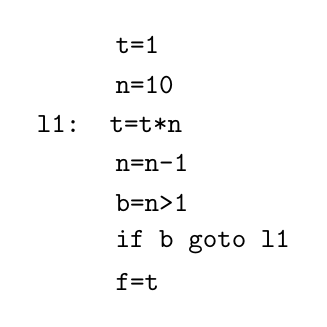
\begin{tikzpicture}
    \node[anchor=west] at ($0*(0,-0.5)$) {\texttt{t=1}};
    \node[anchor=west] at ($1*(0,-0.5)$) {\texttt{n=10}};
    \node[anchor=west] at ($2*(-0.5,-0.5)$) {\texttt{l1: t=t*n}};
    \node[anchor=west] at ($3*(0,-0.5)$) {\texttt{n=n-1}};
    \node[anchor=west] at ($4*(0,-0.5)$) {\texttt{b=n>1}};
    \node[anchor=west] at ($5*(0,-0.5)$) {\texttt{if b goto l1}};
    \node[anchor=west] at ($6*(0,-0.5)$) {\texttt{f=t}};
   \end{tikzpicture}
  & $\Rightarrow$ &
   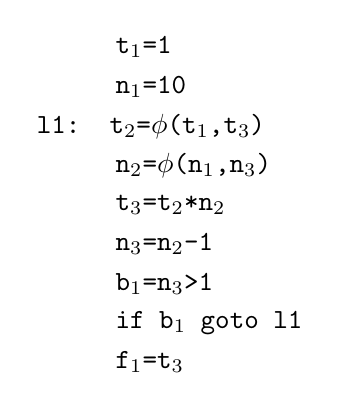
\begin{tikzpicture}
    \node[anchor=west] at ($0*(0,-0.5)$) {\texttt{t$_1$=1}};
    \node[anchor=west] at ($1*(0,-0.5)$) {\texttt{n$_1$=10}};
    \node[anchor=west] at ($2*(-0.5,-0.5)$) {\texttt{l1: t$_2$=$\phi$(t$_1$,t$_3$)}};
    \node[anchor=west] at ($3*(0,-0.5)$) {\texttt{n$_2$=$\phi$(n$_1$,n$_3$)}};
    \node[anchor=west] at ($4*(0,-0.5)$) {\texttt{t$_3$=t$_2$*n$_2$}};
    \node[anchor=west] at ($5*(0,-0.5)$) {\texttt{n$_3$=n$_2$-1}};
    \node[anchor=west] at ($6*(0,-0.5)$) {\texttt{b$_1$=n$_3$>1}};
    \node[anchor=west] at ($7*(0,-0.5)$) {\texttt{if b$_1$ goto l1}};
    \node[anchor=west] at ($8*(0,-0.5)$) {\texttt{f$_1$=t$_3$}};
   \end{tikzpicture} 
 \end{tabular}
\end{document}
